%%%%%%%%%%%%%%%%%%%%%%%%%%%%%%%%%%%%%%%%%%%%%%%%%%%%%%%%%%%%%%%%%%%%%%%%%%%%%%%%%%%%%%%%%%%
% Original author of template for CV (Plasmati Graduate CV v1.0 24/03/2013):
%  Alessandro Plasmati (alessandro.plasmati@gmail.com)
% Changes from the template onwards by (latest 30/01/2019):
% Pol del Aguila Pla (poldap@kth.se)
% Changes from the template onwards by (latest 14/02/2020):
% Joaquim Campos (joaquimcampos@duck.com)
% Downloaded from:
%  http://www.LaTeXTemplates.com
% License:
%  CC BY-NC-SA 3.0 (http://creativecommons.org/licenses/by-nc-sa/3.0/)
% Important note (PdaP):
%  This template needs to be compiled with XeLaTeX.
%  The main document font is called Fontin and can be installed in sudo-enabled
%  Linux systems by running fixFONTproblem.sh (will internally call sudo when necessary).
%%%%%%%%%%%%%%%%%%%%%%%%%%%%%%%%%%%%%%%%%%%%%%%%%%%%%%%%%%%%%%%%%%%%%%%%%%%%%%%%%%%%%%%%%%

%----------------------------------------------------------------------------------------
%	PACKAGES AND OTHER DOCUMENT CONFIGURATIONS
%----------------------------------------------------------------------------------------

% Font and paper size
\documentclass[a4paper,11pt]{article}

% Font loading
\usepackage{fontspec}
  \defaultfontfeatures{Mapping=tex-text}
  % Set main font for document
  \setmainfont[SmallCapsFont = Fontin SmallCaps]{Fontin}
\usepackage{bm}

% Formatting
\usepackage{xunicode,xltxtra,url,parskip}

% Coloring
\usepackage[usenames,dvipsnames]{xcolor}

% Margin specification
\usepackage{fullpage}

% Links and other clickable references
\usepackage{hyperref}
  % Link colors
  \definecolor{linkcolour}{rgb}{0,0.2,0.6}
  \hypersetup{colorlinks,breaklinks,urlcolor=linkcolour,linkcolor=linkcolour}

% Costumize section command
\usepackage{titlesec} % Used to customize the \section command
  % Text formatting
  \titleformat{\section}{\Large\scshape\raggedright}{}{0em}{}[\titlerule]
  % Spacing
  \titlespacing{\section}{0pt}{3pt}{3pt}

% Insert images
\usepackage{graphicx}

% Footnotes in tables
\usepackage{footnote}

% Tables that can span several pages
\usepackage{longtable}

% Several biblographies
\usepackage{bibunits}

% Trademark symbol
\usepackage{textcomp}

% enumerations
\usepackage{enumitem}

% Put references sections in the TOC (PDF and HTML links)
\usepackage[nottoc,numbib]{tocbibind}

\def\myname{Joaquim Campos}


\begin{document}

  % Remove page numbers
  \pagestyle{empty}

  %----------------------------------------------------------------------------------------
  %	NAME AND CONTACT INFORMATION
  %----------------------------------------------------------------------------------------

  \begin{center}
    \begin{tabular}{lcr}
	    \par{\centering{\Huge Joaquim \textsc{Campos}}\bigskip\par} & & 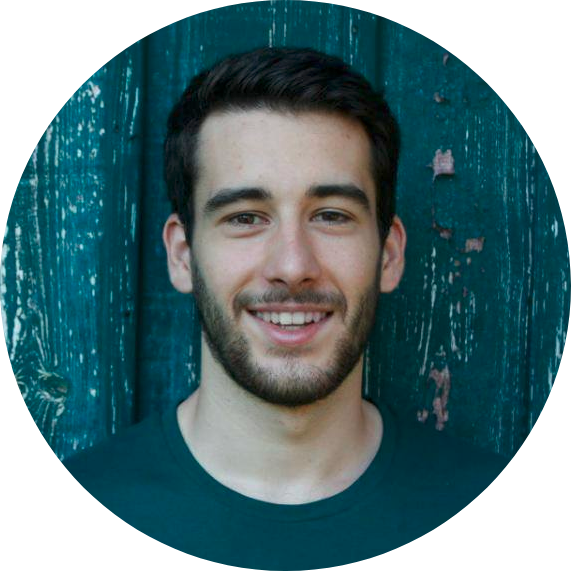
\includegraphics[width=0.3\textwidth]{../../images/Joaquim_circle.png} \\
    \end{tabular}
  \end{center}

  \vspace{15pt}

  \section{Personal data}

    \begin{tabular}{rl}
      \textsc{Place and date of birth:} & Lisbon, Portugal, on 10 February 1996 \\
      % \textsc{Home address:} & Travessa da Cruz da Rocha 3, 4200-344, Porto, Portugal \\
      % \textsc{Mobile phone:} & +351 91-083-2298 \\
      \textsc{Website:} & \url{https://joaquimcampos.com} \\
      \textsc{Email:} & \href{mailto:joaquimcampos@duck.com}{\nolinkurl{joaquimcampos@duck.com}} \\
      \textsc{Google scholar:} & \url{https://scholar.google.com/citations?user=GT-VCroAAAAJ} \\
      % \textsc{Github:} & \url{https://github.com/joaquimcampos} \\
      \textsc{Linkedin:} & \url{https://www.linkedin.com/in/joaquim-campos} \\
    \end{tabular}

  %----------------------------------------------------------------------------------------
  %  Summary
  %----------------------------------------------------------------------------------------

  \vspace{15pt}

  \section{In Brief}
    I am an electrical and computer enginner, programmer, and researcher specialized in signal processing and artificial intelligence. Professionally, I have engaged with deep learning, learning theory, image and video compression, and inverse problems. Outside the scope of my scientific expertise, I dedicate my time to exploring philosophy, psychology, meditation, ethics, and social systems. I find joy in tackling problems holistically, drawing inspiration from both ancient and modern wisdom, and considering the entire pipeline from philosophical and scientific inquiry to practical application. I appreciate engaging in thoughtful discussions, being exposed to different points of view, and—when suitable—sharing the little I know with others.

  %----------------------------------------------------------------------------------------
  %	EDUCATION
  %----------------------------------------------------------------------------------------

  \vspace{15pt}

  \section{Education}

    \begin{tabular}{r|p{13cm}}

      \textsc{\phantom{5}2016 Jul} &
      %
      MSc in \textbf{Applied Buddhist Studies}. \\
      \textsc{Present} &  \footnotesize{\textbf{Tergar Institute}, Kathmandu, Nepal.} \\
      & \footnotesize{
        Program on Buddhist philosophy and meditation. Head Teacher: Mingyur Rinpoche.
        Master's project: \emph{Communicating Madhyamaka Philosophy}.
      } \\
      % 
      \multicolumn{2}{c}{} \\

      %------------------------------------------------

      \textsc{2020 Feb}  &
      %
      MSc in \textbf{Communication Systems}. \\
      \textsc{2016 Sep} & Specialization: \textbf{Signals, Images and Interfaces}. \\
      & \footnotesize{\textbf{École Polytechnique Fédérale de Lausanne}, School of Computer Science and Communication Sciences, Lausanne, Switzerland.} \\
      & \footnotesize{
      % Supervisors and examiner: \textbf{Prof. Michael Unser, Shayan Aziznejad and Prof. François Fleuret}.
      Grade: $\bm{5.67/6.00}$.} — Ranking: 2nd/31 \\
      & \footnotesize{
        Focus on signal processing and artificial intelligence.
        % and their applications to imaging and audio
        Master's thesis: \emph{Higher-Order Regularization Methods for Supervised Learning}. 
        % Biomedical Imaging Group.
      } \\
      %
      \multicolumn{2}{c}{} \\

      %------------------------------------------------
      \textsc{\phantom{5}2016 Jul} &
      %
      BSc in \textbf{Electrical and Computer Engineering}. \\
      \textsc{2013 Sep} &  \footnotesize{\textbf{Universidade de Lisboa}, \emph{Instituto Superior Técnico}, Lisbon, Portugal.} \\
      & \footnotesize{Grade: $\bm{16.4/20.0}$}
    \end{tabular}


  %----------------------------------------------------------------------------------------
  %  WORK EXPERIENCE
  %----------------------------------------------------------------------------------------

  \vspace{15pt}

  \section{Work experience}

    \begin{tabular}{r|p{13cm}}

      \textsc{2023 Dec} 	& Co-Founder and CTO at Radiobooks. \\
      \textsc{2022 Aug} 	& \emph{Converting books into audiobooks automatically using Artificial Intelligence}
      \begin{itemize}[leftmargin=*,noitemsep]
          \item \footnotesize{Designed and created an app for revising AI-generated audio.}
      \end{itemize} \vspace*{-\baselineskip}\\
      \multicolumn{2}{c}{} \\

      %------------------------------------------------

      \textsc{2021 Sep} 	& Research and Teaching Assistant \\
      \textsc{2020 Apr} 	& Topic: \emph{Supervised Learning with Sparsity-Promoting Regularization} \\
				& \footnotesize{ Biomedical Imaging Group, \textbf{École Polytéchnique Fédérale de Lausanne}, Lausanne, Switzerland. Supervisor: \textbf{Prof. Michael Unser}.
				  }
        \begin{itemize}[leftmargin=*,noitemsep]
          \item \footnotesize{Developed a novel framework to learn the activation functions of a neural network;}
          \item \footnotesize{Designed a spline-based supervised learning method which constructs piecewise-linear models with few regions (sparse).}
        \end{itemize} \vspace*{-\baselineskip}\\
      \multicolumn{2}{c}{} \\

      %------------------------------------------------
      \textsc{2018 Aug} & Research Intern \\
      \textsc{2019 Mar} & Topic: \emph{Image and Video Compression using Deep Learning} \\
				& \footnotesize{\textbf{Disney Research}, Zurich, Switzerland. Supervisors: \textbf{Dr. Christopher Schoers and Dr. Abdelaziz Djelouah}.}
        \begin{itemize}[leftmargin=*,noitemsep]
          \item \footnotesize{
            Developed the first content-adaptive neural image compression scheme;}
          \item  \footnotesize{
            Aided in the construction of a state-of-the-art neural video compression framework.}
          \end{itemize} \vspace*{-\baselineskip}

    \end{tabular}

  
  %
  %----------------------------------------------------------------------------------------
  %	TEACHING EXPERIENCE
  %----------------------------------------------------------------------------------------

  \vspace{15pt}

  \section{Teaching experience}

    \begin{tabular}{r|p{13cm}}

	  \textsc{Current}     & Teaching assistance in the courses \textbf{MICRO-310/11: Signals and Systems I/II} \\
	  \textsc{2020 Sep} & \footnotesize{\textbf{École Polytéchnique Fédérale de Lausanne}, Lausanne, Switzerland} \\
    & \footnotesize{Taught by \textbf{Prof. Michael Unser} to the \emph{Life Sciences} and \emph{Microenginneering} sections.} \\
    % & \footnotesize{Approximate numbers per semester:
    %           $250$ students;
    %           $65\,\mathrm{h}$ of guidance of exercise sessions and interaction with students on the course forum;
    %           $60\,\mathrm{h}$ of class preparation; and
		% 					$40\,\mathrm{h}$ of exam supervision and grading.
    %           } \\

    \multicolumn{2}{c}{} \\

    \textsc{Current}	 & Supervision of Master semester projects \\
    \textsc{2020 Sep}  & \footnotesize{\textbf{École Polytéchnique Fédérale de Lausanne}, Lausanne, Switzerland} \\
    & \footnotesize{Co-supervisor of two Master semester projects on \href{https://bigwww.epfl.ch/teaching/projects/abstract.html?f=00388}{lipschitz-constrained generative adversarial networks (GANs)}.} \\

    \end{tabular}

    %----------------------------------------------------------------------------------------
    %	LANGUAGES
    %----------------------------------------------------------------------------------------

    \vspace{15pt}

    \section{Languages}

      \begin{tabular}{rp{10cm}}

        \textsc{Mother tongue:} & Portuguese \\

        \textsc{Professional (C1):} & English \\

        \textsc{Advanced (B2):} & Spanish \\

        \textsc{Conversational (B1):} & French \\

      \end{tabular}

    %----------------------------------------------------------------------------------------
    %	COMPUTER SKILLS
    %----------------------------------------------------------------------------------------

    \vspace{15pt}

    \section{Other skills}

    \begin{tabular}{rp{11cm}}
  	Primary technical skills:  & Knowledge of both theoretical and practical aspects of signal processing, machine learning, and deep learning.
    \vspace{5pt}\\
  	Programming:       &  \textsc{C, Python, FastAPI, PyTorch, Bash, Matlab, \LaTeX, Backend development and deployment}  \vspace{5pt} \\
  	Other skills: 	   & During my academic years, I developed valuable presentation, writing, and teaching skills, much of which I owe to Prof. Michael Unser.

    \end{tabular}

  %----------------------------------------------------------------------------------------
  %	PUBLICATIONS AND PATENTS
  %----------------------------------------------------------------------------------------

  % \newpage

  The publications can be consulted here: \url{https://joaquimcampos.com/pubs.html}. \\[5pt]

  \begin{bibunit}[IEEEtran_Pol]
    \renewcommand\refname{Publications: Science}

    \nocite{
      goujonStableParameterizationContinuous2023,
      aziznejadMeasuringComplexityLearning2023,
      camposLearningContinuousPiecewiseLinear2022,
      bohraLearningActivationFunctions2020,
      aziznejadDeepNeuralNetworks2020,
      djelouahNeuralInterFrameCompression2019,
      camposContentAdaptiveOptimization2019}
    \putbib[../pubs/bibfile]

  \end{bibunit}

  \vspace{20pt}

  \begin{bibunit}[IEEEtran_Pol]
    \renewcommand\refname{Publications: Philosophy}

    \nocite{
      camposMahayanaBuddhistEthicsWork-in-Progress,
      camposWrongnessKillingNonHuman2018} %
    \putbib[../pubs/bibfile]

  \end{bibunit}

  \vspace{20pt}

  \begin{bibunit}[IEEEtran_Pol]
    \renewcommand\refname{Patents}

    \nocite{
      schroersContentAdaptiveOptimization2021,
      schroersSystemsMethodsReconstructing2021,
      schroersSystemsMethodsGenerating2021}
    \putbib[../pubs/bibfile]

  \end{bibunit}

  %----------------------------------------------------------------------------------------
  % INTERESTS AND ACTIVITIES
  %----------------------------------------------------------------------------------------

  % \vspace{-5pt}
  %
  % \section{Interests and activities}
  %
  % \section{On a Personal Note}
  %
  %   I meditate every morning. Cold showers clear my mind. Reader, especially about personal development, philosophy, psychology and society. When I have time a Pixar or Studio Ghibli movie, do Yoga or dancing. Productivity. I shut my cellphone during work and don't touch it on sundays. I practice a vegan lifestyle. I like to think deeply about topics and question my assumptions and beliefs. I work to be a positive influence am mindful of treating others with respect and compassion. I like to have my mind changed and engage in a healthy discussion. I have been fortunate enough to have traveled to abroad every year since I remember. I did competitive volleyball for $10$ years, swimming and represented Portugal at the I represented Portugal at the Youth World Padel Tournament in Mellilla in 2011. Music runs is a passion Piano or Guitar – 4 and 7 years of lessons, respectively.\\
  %
  % \section{Book list}
  %
  % \begin{tabular}{rp{10cm}}
  %
  %   \emph{The Righteous Mind} & by Jonathan Haidt \\
  %
  %   \emph{Animal Liberation} & by Peter Singer \\
  %
  % \end{tabular}
  %
  % \section{Traits}
  %
  % \begin{tabular}{rp{10cm}}
  %
  %   \emph{The Righteous Mind} & by Jonathan Haidt \\
  %
  %   \emph{Animal Liberation} & by Peter Singer \\
  %
  % \end{tabular}

\end{document}
